\chapter{État de l'art}
\label{chap:etat_art}

% ---------------------------------------------------------------
% ---------------------------------------------------------------
\section{Model-Driven Engineering}
\label{sec:mde}
% ---------------------------------------------------------------
% ---------------------------------------------------------------

L'émergence de l'Ingénierie Dirigée par les Modèles (MDE) répond à la nécessité de simplifier le développement de systèmes logiciels complexes et d'automatiser leurs cycles de production. En plaçant les modèles au centre du processus d'ingénierie, cette approche facilite le partage d'une vision et de connaissances communes entre les parties prenantes techniques et non techniques~\cite{da2015model}. L'évolution vers la MDE permet également de s'abstraire des complexités liées aux environnements informatiques sous-jacents en privilégiant des langages et des plateformes de plus haut niveau~\cite{schmidt2006model}. Cette élévation du niveau d'abstraction repose sur une séparation rigoureuse des préoccupations : les architectes peuvent ainsi se concentrer sur les décisions métier essentielles, indépendamment des spécificités et des fluctuations des technologies cibles~\cite{brown2004model}.

Pour représenter fidèlement des systèmes d'envergure, une approche multi-modèles est généralement indispensable~\cite{brown2004model,da2015model}. Chaque modèle offre une vue partielle et simplifiée, se focalisant sur des perspectives spécifiques (structurelle, comportementale ou physique) afin de maîtriser la complexité croissante des solutions d'entreprise.

La MDE englobe diverses méthodologies telles que l'Architecture Dirigée par le Modèle (MDA), les Software Factories ou l'ingénierie des Domain Specific Languages (DSL). Bien que ces approches diffèrent dans leurs objectifs et leurs outils, elles s'appuient sur des techniques avancées telles que la méta-modélisation, la transformation de modèles et la génération de code pour automatiser la création ou l'exécution de systèmes~\cite{da2015model}.

% ---------------------------------------------------------------
\subsection{CASE et MetaCASE}
\label{sec:case-metacase}
% ---------------------------------------------------------------

Les premiers outils utilisés pour automatiser les tâches de conception et de documentation sont les outils CASE (Computer-Aided Software Engineering). Ces outils supportent généralement un nombre fixe de méthodologies (comme UML ou les diagrammes de flux de données) qui sont codées en dur par le fournisseur. Dans un outil CASE standard, l'architecture est à deux niveaux : les conceptions système sont stockées dans un référentiel dont le schéma est figé~\cite{isazadeh1997case}. Cette rigidité est l'un des principaux freins à l'adoption de méthodologies innovantes ou spécifiques à un domaine, car seul le vendeur peut modifier le fonctionnement de l'outil.

Les technologies MetaCASE approchent l'automatisation de manière dynamique. Elles permettent de générer dynamiquement des environnements de modélisation adaptés à n'importe quelle méthode ou domaine. Les MetaCASE reposent sur une architecture à trois niveaux (voir figure \ref{isa-fig}) où le métamodèle de la méthode n'est pas programmé dans le code source de l'outil, mais stocké comme une donnée modifiable dans le référentiel~\cite{isazadeh1997case}.
\begin{itemize}
    \item Niveau Meta : les développeurs construisent les composants génériques et définissent le méta-modèle.
    \item Niveau Environnement : le méta-modèle est utilisé pour bâtir un outil CASE spécifique à l'organisation.
    \item Niveau Utilisateur : les développeurs utilisent cet outil sur mesure pour créer les produits logiciels.
\end{itemize}
\begin{figure}[h]
\centering
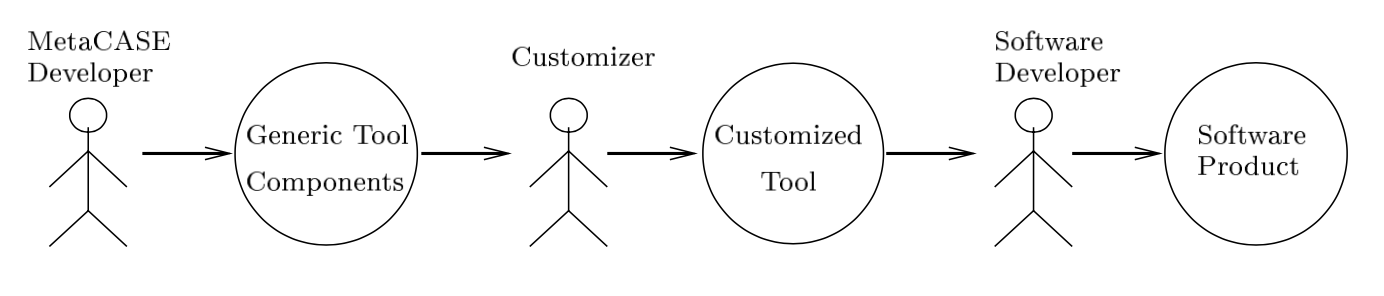
\includegraphics[width=0.8\textwidth]{img/etat_art/metacase3level.png}
\caption{Vue d'ensemble des 3 niveaux d'architecture MetaCASE~\cite{isazadeh1997case}}
\label{isa-fig}
\end{figure}
MetaDONE s'inscrit pleinement dans cette architecture à trois niveaux, en proposant un framework méta générique, un mécanisme de définition d'environnements CASE par méta-modélisation et un niveau utilisateur pour la création de modèles concrets.

% ---------------------------------------------------------------
% ---------------------------------------------------------------
\section{Langages de modélisation}
\label{sec:langages}
% ---------------------------------------------------------------
% ---------------------------------------------------------------

La MDE repose sur l'utilisation de langages de modélisation pour exprimer les différentes facettes d'un système. Ces langages se distinguent par leur niveau de généralité~: certains visent une applicabilité universelle tandis que d'autres ciblent un domaine précis. Comprendre cette distinction est essentiel pour saisir pourquoi des outils comme MetaDONE ont été conçus, et quelles contraintes techniques leur usage impose.

% ---------------------------------------------------------------
\subsection{Langages généraux de modélisation}
\label{sec:langages-generaux}
% ---------------------------------------------------------------

Les premiers langages à s'imposer dans le contexte MDE sont des langages à usage général (\textit{General Purpose Modeling Languages}, GPL), dont le représentant le plus emblématique est UML (\textit{Unified Modeling Language}). Adopté comme standard par l'OMG\footnote{Object Management Group, \url{https://www.omg.org}}, UML a été conçu pour unifier les nombreuses pratiques de modélisation alors en vigueur dans l'industrie~\cite{france2007mde}. 
\begin{wrapfigure}{r}{5.5cm}
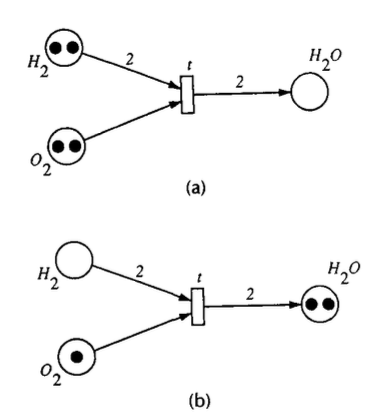
\includegraphics[width=5.5cm]{img/etat_art/petri.png}
\caption{Exemple d'illustration de la réaction chimique $2H_2 + 0_2 \rightarrow 2H_20$ avec les réseaux de Petri~\cite{murata1989petri}}
\label{murata-fig}
\end{wrapfigure} 
Sa force réside dans sa polyvalence~: il couvre les aspects structurels (diagrammes de classes, de composants), comportementaux (machines à états, diagrammes de séquence) et de déploiement d'un système logiciel.

Cependant, cette généralité devient rapidement un frein. En cherchant à tout couvrir, UML est devenu extrêmement large et complexe. De plus, il ne permet pas de définir entièrement les relations entre ses propres diagrammes, et la spécification de comportements détaillés y reste difficile~\cite{koshima2016distributed}. Le mécanisme d'extension officiel d'UML, les \textit{profils}, est largement reconnu comme insuffisant~: il ne permet que d'adapter superficiellement la syntaxe du langage, sans modifier le métamodèle ni la sémantique sous-jacente~\cite{Eng2007}.


À côté d'UML, les \textbf{réseaux de Petri} constituent un autre langage de modélisation à usage général, orienté cette fois vers la spécification formelle de systèmes concurrents et distribués~\cite{reisig1985petri,murata1989petri}. Un réseau de Petri est défini par un ensemble de \textit{places} (états potentiels du système), de \textit{transitions} (événements pouvant survenir) et d'\textit{arcs orientés} les reliant. Des \textit{jetons} circulent dans le réseau pour représenter l'état courant du système (voir exemple figure \ref{murata-fig}). Leur sémantique formelle bien établie les rend particulièrement adaptés à l'analyse de propriétés telles que la vivacité, la sûreté ou l'absence d'interblocage. Ils servent d'ailleurs d'exemple canonique dans la documentation de MetaDONE pour illustrer la définition d'un métamodèle avec MetaL$_2$~\cite{techreportgrasylaversion2}.

Si ces deux langages partagent l'ambition d'être universellement applicables, ils souffrent d'une limite commune~: en voulant s'adapter à tous les domaines, ils n'en servent aucun de manière optimale. Un expert métier confronté à un diagramme de classes UML ou à un réseau de Petri doit d'abord maîtriser le formalisme avant de pouvoir exprimer ses connaissances. C'est précisément cette friction qui a motivé l'émergence des langages spécifiques au domaine.

% ---------------------------------------------------------------
\subsection{Domain Specific Languages et DSML}
\label{sec:dsl-dsml}
% ---------------------------------------------------------------

Face aux limites des GPL, une approche complémentaire s'est imposée~: la conception de \textit{Domain Specific Languages} (DSL), c'est-à-dire des langages de modélisation conçus pour un domaine applicatif précis plutôt que pour une utilisation générale~\cite{schmidt2006model}. Lorsqu'un tel langage est doté d'un métamodèle explicite constituant sa syntaxe abstraite, d'une notation concrète (textuelle ou graphique) et d'une sémantique formalisée, on parle de \textit{Domain Specific Modeling Language} (DSML)~\cite{koshima2016distributed}.

La distinction fondamentale entre un modèle et son langage repose sur la séparation entre \textbf{syntaxe abstraite} et \textbf{syntaxe concrète}. La syntaxe abstraite décrit les concepts du langage et leurs relations~; elle est spécifiée par un métamodèle. La syntaxe concrète est la surface visible par l'utilisateur~: la notation graphique, textuelle ou mixte avec laquelle il interagit~\cite{koshima2016distributed}. Dans MetaDONE, GraSyLa (\textit{Graphical Symbolic Language}) joue précisément ce rôle de pont entre syntaxe abstraite et syntaxe concrète~: c'est un DSML dédié à la définition des notations concrètes à partir des métamodèles MetaL$_2$~\cite{techreportgrasylaversion2}.

L'intérêt principal d'un DSML est de permettre aux experts du domaine de travailler directement avec leurs propres concepts, sans devoir maîtriser une technologie de modélisation générique~\cite{koshima2016distributed}. En conséquence, la qualité des produits logiciels s'améliore, les coûts de conception et de développement diminuent, et la longévité des systèmes augmente~\cite{koshima2016distributed}. Des études empiriques suggèrent que l'adoption de DSML peut améliorer la productivité d'un facteur cinq à dix par rapport aux approches par langage général~\cite{kelly2008dsm}.


\begin{wrapfigure}{l}{3.8cm}
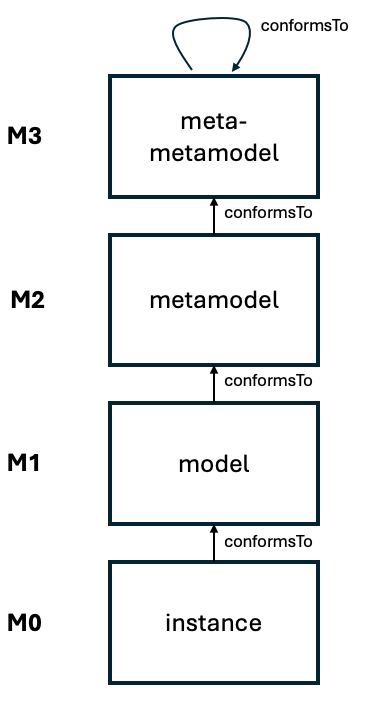
\includegraphics[width=3.5cm]{img/etat_art/omg4level.png}
\caption{Représentation des 4 niveaux d'abstraction de l'OMG}
\label{fig:omf4level}
\end{wrapfigure} 
Du point de vue de l'architecture MDE, un DSML est lui-même un modèle~: il est conforme à un \textit{métamodèle} (qui en définit la structure), lequel est conforme à un \textit{métamétamodèle} (qui définit le langage de métamodélisation lui-même). Cette hiérarchie à trois niveaux --- model, meta-model, meta-meta-model --- est représentée dans l'architecture à quatre couches de l'OMG (M0 à M3), dont MOF (\textit{Meta Object Facility}) constitue le niveau supérieur~\cite{da2015model} (voir figure~\ref{fig:omf4level}). MetaDONE adopte une approche analogue, supportant les niveaux M1, M2 et M3 de la hiérarchie OMG au sein d'un même environnement réflexif~\cite{Eng2007}.


Il convient de noter que les outils MetaCASE et les environnements DSM (\textit{Domain-Specific Modeling}) modernes reposent sur des \textit{Metamodeling Languages} (MML) — comme MOF, Kermeta, KM3 ou GOPPRR — pour définir leurs DSL. Ces langages présentent cependant plusieurs limitations communes~: l'incapacité ou la difficulté à établir des liens entre des construits sémantiquement liés répartis dans des (méta)modèles distincts~; la restriction des niveaux de modélisation éditables, généralement limités à M2 (méta-modèle) et M1 (modèle); l'impossibilité pour les relations de traverser les frontières entre niveaux d'abstraction, connue sous le nom de \textit{strict metamodelling}; et le codage en dur de diverses informations — le MML lui-même, des éléments de syntaxe concrète, l'interface graphique ou les mécanismes de versionnement~\cite{Eng2007}.

% ---------------------------------------------------------------
\section{Tour d'horizon des outils MetaCASE}
\label{sec:metacase-outils}
% ---------------------------------------------------------------

La prolifération des DSML dans l'industrie a conduit au développement d'outils MetaCASE capables de les générer dynamiquement à partir de métamodèles. Bien que ces outils partagent l'architecture à trois niveaux décrite à la section~\ref{sec:case-metacase}, leurs choix de conception les différencient significativement~\cite{Eng2007}. Nous retenons ci-dessous trois outils représentatifs des principales familles d'approches~: MetaEdit+ pour sa maturité industrielle, WebGME pour sa dimension collaborative web, et ConceptBase pour son langage à axiomes flexibles~; chacun éclaire, par contraste, les choix de conception de MetaDONE.

\textbf{MetaEdit+}~\cite{kelly1996metaedit+} est l'un des outils MetaCASE les plus matures industriellement. Il repose sur le langage de métamodélisation GOPPRR (\textit{Graph, Object, Property, Port, Role, Relationship}) et permet le partage de propriétés entre métamodèles. Il offre un support solide pour la modélisation collaborative via un mécanisme de verrouillage fin (\textit{Smart Locks}), mais sa flexibilité reste contrainte~: il n'autorise pas les relations entre niveaux d'abstraction distincts (\textit{strict metamodelling}) et limite le nombre de niveaux M à deux ou trois.

\textbf{WebGME} (\textit{Web-based Generic Modeling Environment})~\cite{webgme} est l'évolution web de GME~\cite{ledeczi2001generic}, un environnement MetaCASE historiquement utilisé dans les domaines de l'embarqué et du génie système. Là où GME reposait sur une application de bureau monoposte, WebGME est une plateforme collaborative hébergée dans le navigateur, offrant l'édition simultanée par plusieurs utilisateurs, un système de versionnement par branches similaire à celui du code source, et une API JavaScript/REST permettant l'intégration avec des outils externes. La définition de DSMLs repose sur un métamodèle de style UML que l'outil interprète pour se configurer automatiquement, et un mécanisme d'héritage prototypique propage les modifications d'un prototype à ses instances. WebGME conserve toutefois la limitation à trois niveaux M et le \textit{strict metamodelling} hérités de GME.

\textbf{ConceptBase}~\cite{jeusfeld2005meta} adopte une approche différente en s'appuyant sur Telos, un langage de métamodélisation très flexible autorisant un nombre de niveaux illimité et un \textit{non-strict metamodelling} (les relations peuvent traverser les niveaux d'abstraction). Sa principale force est un langage déclaratif puissant pour exprimer des contraintes, des règles et des requêtes. Cependant, ses capacités graphiques sont limitées comparées à GraSyLa, et ses axiomes plus rigides que ceux de MetaL~\cite{Eng2007}.

\textbf{MetaDONE}~\cite{Eng2007} se distingue par sa philosophie entièrement \textit{model-driven}~: chaque aspect de l'outil est lui-même un modèle conforme à un métamodèle. Cette propriété, combinée à la \textit{réflexivité universelle} de MetaL, autorise un bootstrapping progressif des fonctionnalités~: l'interface graphique, les notations concrètes, et le contrôle de version peuvent tous être définis ou étendus sans modifier le code source de l'outil. MetaDONE dépasse la limitation des trois niveaux M et permet aux relations de traverser les niveaux d'abstraction (\textit{non-strict metamodelling}). Son dépôt est technologiquement indépendant~: il peut fonctionner avec JDO, RDF ou XMI comme backend de persistance~\cite{Eng2007}. En contrepartie, cette flexibilité engendre une multiplication des couches d'indirection dont le coût en performances doit être évalué et maîtrisé~\cite{Eng2007} --- ce qui constitue l'objet de ce mémoire.

Le tableau~\ref{tab:metacase} synthétise les principales différences de ces MetaCASE.

\begin{table}[h]
\centering
\caption{Comparaison des principaux outils MetaCASE}
\label{tab:metacase}
\small
\begin{tabular}{lllll}
\hline
\textbf{Outil} & \textbf{MML} & \textbf{Niveaux M} &
\textbf{Non-strict} & \textbf{Réflexivité} \\
\hline
MetaEdit+   & GOPPRR    & 2--3      & Non & Non \\
WebGME      & UML-like  & 3         & Non & Non \\
ConceptBase & Telos     & Illimités & Oui & Partielle \\
MetaDONE    & MetaL     & Illimités & Oui & Totale \\
\hline
\end{tabular}
\end{table}

La réflexivité totale de MetaL, qui fait la force de MetaDONE, a une conséquence structurelle directe~: elle augmente la densité du graphe de données stockées dans le dépôt ainsi que la complexité computationnelle des algorithmes de parcours et de gestion. Cette propriété, bénéfique pour l'expressivité du langage, introduit des contraintes spécifiques dès lors qu'il s'agit de sérialiser ou de charger ces données en mémoire. La section suivante examine en détail la nature de ces graphes et leurs implications pour la persistance.

% ---------------------------------------------------------------
% ---------------------------------------------------------------
\section{Les modèles comme graphes}
\label{sec:graphes}
% ---------------------------------------------------------------
% ---------------------------------------------------------------

Les sections précédentes ont présenté la MDE et ses langages de modélisation de manière conceptuelle. Pour comprendre les enjeux de performance propres à MetaDONE, il est nécessaire de descendre au niveau de la représentation concrète des données~: tout modèle MDE est fondamentalement une structure de graphe, et les propriétés particulières du graphe de MetaL engendrent des contraintes techniques spécifiques sur la persistance et le chargement en mémoire.

% ---------------------------------------------------------------
\subsection{Structure en graphe d'un modèle MDE}
\label{sec:graphes-mde}
% ---------------------------------------------------------------

Dans le contexte de la MDE, un modèle peut être formellement représenté comme « un graphe composé de concepts et de relations entre ces concepts »~\cite{bezivin2005model}. Les nœuds correspondent aux objets (instances de méta-objets) et les arêtes aux relations entre ces objets (instances de méta-rôles). Cette représentation est universelle~: un diagramme de classes UML, un réseau de Petri, ou un métamodèle MetaL$_2$ s'expriment tous dans ce même formalisme.

Dans MetaL$_1$, la couche formelle de base de MetaDONE détaillée au chapitre~\ref{chap:architecture}, le dépôt est un ensemble $D$ de \textit{DataObjects}~\cite{englebert_metal1}. Chaque DataObject peut acquérir un ensemble de \emph{facettes} qui déterminent son rôle dans le graphe~: un DataObject portant la facette \emph{Object} appartient à l'ensemble $O$ des objets, un DataObject portant la facette \emph{Property} appartient à l'ensemble $P$ des propriétés. Ces deux ensembles ne sont pas disjoints~--- un même DataObject peut porter simultanément les deux facettes, devenant ainsi à la fois un objet et une propriété~\cite{Eng2007}. Une propriété possède un domaine (\textit{domain}) et un codomaine (\textit{range}) qui sont tous deux des objets~: les propriétés sont donc des arêtes orientées dans le graphe du dépôt. Les relations de spécialisation (\texttt{isa}) et d'instanciation (\texttt{instanceOf}) constituent des arêtes supplémentaires dans ce graphe.

Cette représentation unifiée est un atout majeur de MetaL~: elle permet de traiter de manière homogène les objets, les types, les métaobjets et les métamodèles au sein d'un unique graphe persisté dans le dépôt.

% ---------------------------------------------------------------
\subsection{Graphes cycliques et réflexivité}
\label{sec:graphes-cycliques}
% ---------------------------------------------------------------

La plupart des modèles courants --- un diagramme de classes UML ou un réseau de Petri --- forment des graphes dont les cycles sont limités ou inexistants au niveau des relations de typage et de spécialisation. Les outils conventionnels, EMF en tête, reposent sur cette hypothèse~: la relation \texttt{isa} y est supposée acyclique, et la hiérarchie métamodèle/modèle est strictement séparée~\cite{steinberg2008emf}.

MetaL adopte délibérément une position contraire. Sa différence fondamentale avec les autres langages de métamodélisation réside dans son support complet de la \textit{réification}, qui se manifeste notamment par quatre propriétés clés de MetaL$_1$~\cite{Eng2007}~:

\begin{enumerate}
    \item \textbf{Non-disjonction de $O$ et $P$}~: un item peut être à la fois un objet et une propriété. Un \texttt{MetaRole} est ainsi simultanément un type d'objet (il peut être instancié) et un type de propriété (il relie deux objets). Cette dualité crée des arêtes qui sont elles-mêmes des nœuds dans le graphe.
    
    \item \textbf{Absence d'axiome d'acyclicité}~: contrairement aux pratiques courantes, MetaL n'impose pas que la relation \texttt{isa} soit acyclique. Cela permet la spécialisation multiple sans restriction, mais introduit la possibilité de cycles dans le graphe de spécialisation.

    \item \textbf{Instanciation multiple}~: un objet peut être instance de plusieurs types simultanément. Dans l'exemple documenté par Englebert et Heymans, \textit{Mainframe Fenris} est à la fois un nœud de déploiement et une classe de conception~\cite{Eng2007}. Cette caractéristique crée des arêtes \texttt{instanceOf} en étoile autour d'un même nœud.

    \item \textbf{Réflexivité de la relation \texttt{instanceOf}}~: c'est la propriété la plus structurante. Tout DataObject séminal de MetaL$_1$ est instance de lui-même~\cite{englebert_metal1}. À l'échelle de MetaL$_2$, cela signifie que chacune des métaclasses fondamentales (\texttt{MetaObject}, \texttt{MetaModel}, \texttt{MetaRole}, \texttt{MetaProperty}) est instance \emph{d'elle-même}~\cite{englebert_metal2}~: \texttt{MetaObject} est instance de \texttt{MetaObject}, \texttt{MetaRole} est instance de \texttt{MetaRole}, et ainsi de suite. C'est cette propriété~--- absente du MOF où le niveau M3 est seulement « conforme à lui-même »~--- qui permet la méta-circularité totale du système~: le métamétamodèle se décrit ainsi entièrement avec ses propres construits.
\end{enumerate}

La figure~\ref{instanceOf} illustre cette réflexivité au niveau de MetaL$_1$~: les flèches \texttt{instance-of} bouclent sur les items séminaux eux-mêmes, formant des cycles explicites dans le graphe du dépôt.

\begin{figure}[h]
\centering
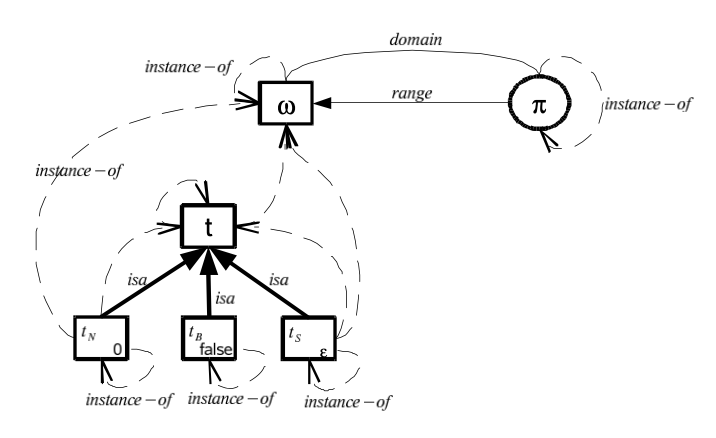
\includegraphics[width=0.7\textwidth]{img/etat_art/instanceOf.png}
\caption{Relations instanceOf réflexives explicites permettant la réification du type de propriété nom en une métapropriété de première classe P~\cite{Eng2007}}
\label{instanceOf}
\end{figure}

Cette méta-circularité est la propriété qui rend possible le \textit{bootstrapping} de MetaDONE. Grâce à elle, toute fonctionnalité de l'outil peut être définie comme un modèle conforme au même métamétamodèle, puis étendue sans modifier le code source~\cite{Eng2007}. GraSyLa lui-même est un DSML implémenté de cette façon~: ses spécifications sont des modèles concrets ordinaires du dépôt~\cite{techreportgrasylaversion2}.


En revanche, cette même propriété est source de défis techniques dès lors qu'il s'agit de \textbf{persister} le graphe du dépôt ou de le \textbf{charger en mémoire}.

% ---------------------------------------------------------------
\subsection{Conséquences pour la persistance}
\label{sec:graphes-persistance}
% ---------------------------------------------------------------

Les deux principales approches de persistance utilisées dans l'écosystème MDE ont été conçues en supposant des modèles essentiellement arborescents ou, au moins, acycliques~: elles rencontrent donc des difficultés structurelles face aux graphes cycliques de MetaL.

Le format XMI (\textit{XML Metadata Interchange}), standard OMG pour la persistance des modèles EMF, repose sur la structure hiérarchique de XML~\cite{specification2007omg}. XML est intrinsèquement arborescent~: chaque élément a exactement un parent, ce qui est incompatible avec un graphe contenant des cycles ou du partage (un nœud ayant plusieurs parents). Pour contourner cette limitation, XMI introduit un mécanisme de références croisées par identifiants (\textit{href})~: les objets partagés ou référencés de manière circulaire sont sérialisés une seule fois à leur point d'ancrage dans l'arbre, et référencés ailleurs par leur identifiant. Ce mécanisme fonctionne pour les modèles conventionnels mais présente des limites importantes dans le cas de MetaL~: la réflexivité totale implique que la quasi-totalité des items du métamétamodèle peuvent être à la fois la cible et la source de références circulaires, ce qui complexifie la détermination d'un ordre de sérialisation valide et impose une résolution de toutes les références lors du chargement avant de pouvoir utiliser le moindre objet. De surcroît, XMI nécessite le chargement intégral du fichier en mémoire avant de pouvoir en extraire une information partielle~\cite{steinberg2008emf}, ce qui le rend peu adapté aux grands modèles.

L'architecture du dépôt de MetaDONE est conçue pour être indépendante de la technologie de persistance sous-jacente~\cite{Eng2007}. L'implémentation courante repose sur OpenJPA qui mappe les objets Java vers un schéma relationnel~\cite{jpa2013}.

Ce mapping soulève un problème fondamental~: si les bases de données relationnelles représentent les données sous forme de tables et de clés étrangères sans difficulté particulière face aux références circulaires au niveau du stockage, les mécanismes de chargement objet-relationnel (ORM) y sont sensibles. Lorsqu'un ORM charge un objet, il doit décider comment charger ses références~: soit immédiatement (\textit{eager loading}), ce qui peut déclencher une cascade infinie en présence de cycles, soit à la demande (\textit{lazy loading}), ce qui reporte le problème à l'accès effectif à la référence. La résolution d'un graphe cyclique lors du chargement requiert donc un mécanisme explicite de détection des objets déjà en cours de chargement~: en garantissant qu'un identifiant donné correspond toujours à la même instance en mémoire, ce mécanisme --- connu sous le nom d'\textit{identity map} ou \textit{first-level cache} --- interrompt la récursion et retourne l'instance partiellement construite. La spécification JPA formalise ce comportement sous le terme \textit{persistence context}~\cite{jpa2013}.

Dans MetaDONE, cette contrainte est accentuée par le fait que les items séminaux de MetaL$_1$ --- qui forment les cycles les plus profonds du graphe --- sont nécessairement présents dans tout projet et constituent donc un point de passage obligé lors de chaque chargement du dépôt.

Les cycles structurels du graphe MetaL ne sont pas gérables par de simples heuristiques~: ils sont au cœur de la conception du langage. Toute stratégie d'optimisation des accès au dépôt de MetaDONE doit en tenir compte explicitement, que ce soit pour le chargement initial en mémoire, la mise en cache des objets fréquemment référencés, ou la stratégie de chargement différé des relations. Ces problématiques de persistance s'inscrivent dans un enjeu plus large de scalabilité du MDE, que la section suivante examine.

% ---------------------------------------------------------------
% ---------------------------------------------------------------
\section{Scalabilité en MDE}
\label{sec:scalabilite-mde}
% ---------------------------------------------------------------
% ---------------------------------------------------------------

Les sections précédentes ont établi que les modèles MDE sont fondamentalement des graphes, et que ceux de MetaDONE présentent la particularité d'être cycliques et denses par construction. Cette réalité structurelle s'inscrit dans un défi plus large que traverse l'ensemble de la communauté MDE depuis une décennie~: celui de la scalabilité. Le passage de modèles locaux de taille modeste à des écosystèmes de modèles interconnectés regroupant des millions d'éléments remet en cause les hypothèses fondatrices des outils MDE traditionnels~\cite{kolovos2013research}. Cette section passe en revue les principales dimensions de ce défi, en se concentrant sur celles qui sont directement pertinentes pour MetaDONE.

% ---------------------------------------------------------------
\subsection{Transformations et requêtes}
\label{sec:transfo-requetes}
% ---------------------------------------------------------------

Les transformations de modèles constituent le cœur opérationnel de la MDE~: elles permettent de générer automatiquement un modèle cible à partir d'un modèle source selon une définition de transformation~\cite{bezivin2005model}. Lorsque la taille des modèles augmente, les performances de ces transformations deviennent un enjeu critique.

Deux techniques complémentaires ont émergé comme réponses principales. La première est l'\textbf{incrémentalité}~: plutôt que de ré-exécuter une transformation sur l'ensemble du modèle à chaque modification, seules les parties affectées par le changement sont recalculées. Des outils comme EMF-IncQuery illustrent cette approche dans l'écosystème EMF~\cite{bergmann2010incremental}. La seconde est le \textbf{calcul différé} (\textit{lazy evaluation})~: les valeurs ne sont calculées qu'au moment où elles sont effectivement nécessaires, évitant ainsi le calcul prématuré de résultats qui ne seront jamais consultés.

Une piste de recherche plus récente consiste à adopter un paradigme \textit{réactif}, dans lequel un réseau de transformations définit des flux de données persistants. Chaque modification d'un modèle source propage automatiquement ses effets aux modèles dépendants, en n'activant que les calculs strictement nécessaires~\cite{cabot2012object}. Ce paradigme est particulièrement adapté aux environnements MetaCASE où les métamodèles et les modèles évoluent de concert.

% ---------------------------------------------------------------
\subsection{Modélisation collaborative}
\label{sec:model-collaborative}
% ---------------------------------------------------------------

La modélisation collaborative constitue une autre dimension de la scalabilité~: lorsque plusieurs utilisateurs travaillent simultanément sur un même modèle, la gestion de la cohérence et des conflits devient un problème d'envergure.

La plupart des outils MDE actuels n'atteignent pas la maturité des systèmes de gestion de versions de code source tels que Git ou SVN. EMFStore offre un support pour l'édition collaborative de modèles et de métamodèles EMF/Ecore, mais ne dispose pas de mécanisme de réconciliation basé sur les rôles et laisse à l'utilisateur ayant effectué le dernier commit la responsabilité de résoudre les conflits~\cite{koshima2016distributed}. MetaEdit+ recourt à un mécanisme de verrouillage fin (\textit{Smart Locks}) pour la gestion de la concurrence, mais les approches par verrou ne passent pas à l'échelle en équipes nombreuses~\cite{koshima2016distributed}. Des frameworks plus récents, comme DiCoMEF~\cite{koshima2016distributed}, proposent des architectures distribuées avec détection et réconciliation formalisées des conflits, mais restent au stade de la recherche.

La modélisation collaborative, bien que pertinente dans le domaine MDE, sort du périmètre de ce mémoire et ne sera pas davantage développée ici.

% ---------------------------------------------------------------
\subsection{Persistance de grands modèles}
\label{sec:persistance-modeles}
% ---------------------------------------------------------------

La persistance est la dimension de la scalabilité la plus directement liée aux objectifs de ce mémoire. Elle désigne la capacité d'un outil MDE à stocker et à charger efficacement des modèles de grande taille, en particulier lorsque ceux-ci présentent une structure complexe comme les graphes cycliques de MetaL.

% ---------------------------------------------------------------
\subsubsection{Limites de XMI}
\label{sec:limites-xmi}
% ---------------------------------------------------------------

Le format XMI (\textit{XML Metadata Interchange}) est le standard industriel de sérialisation des modèles EMF. Sa principale limite tient à sa nature même~: il impose un chargement et une désérialisation intégraux du fichier avant qu'une quelconque requête puisse être exécutée~\cite{steinberg2008emf}. Si la capacité mémoire des machines modernes atténue le problème pour des modèles de taille raisonnable, cette approche reste fondamentalement inefficace~: même une requête ponctuelle (par exemple, retrouver toutes les sous-classes d'un méta-objet donné) nécessite de parcourir l'intégralité du fichier, sans possibilité d'indexation ni d'accès incrémental. Le temps de chargement initial reste par ailleurs significatif pour les grands modèles, indépendamment de la mémoire disponible.

Comme détaillé à la section~\ref{sec:graphes-persistance}, XMI souffre en outre d'une incompatibilité structurelle avec les graphes cycliques~: étant fondé sur XML, il ne peut représenter qu'une arborescence, et doit donc recourir à des références croisées par identifiants pour simuler le partage ou les cycles. Pour les modèles réflexifs de MetaL, où la quasi-totalité des items séminaux sont à la fois instances et types de l'ensemble du graphe, ce mécanisme génère un grand nombre de références à résoudre lors du chargement, dont l'ordre de résolution doit être soigneusement géré.

Des travaux ont proposé de remplacer XMI par des formats binaires comme Google Protocol Buffers, pouvant réduire la taille des fichiers d'un facteur dix et améliorer la vitesse de chargement jusqu'à cent fois pour des modèles de grande taille~\cite{protobuf}. Ces approches restent cependant contraintes par la même hypothèse de chargement intégral en mémoire.

% ---------------------------------------------------------------
\subsubsection{Persistance par base de données avec OpenJPA}
\label{sec:persistance-openjpa}
% ---------------------------------------------------------------

Pour s'affranchir des limites des formats de fichiers, MetaDONE adopte une architecture de dépôt indépendante de la technologie de persistance sous-jacente, permettant de le connecter à différents backends~\cite{Eng2007}. L'implémentation principale repose sur OpenJPA, une implémentation de la Java Persistence API qui assure le mapping entre les objets Java du dépôt et un schéma relationnel.

Cette approche présente plusieurs avantages pour la scalabilité. D'abord, elle permet l'accès partiel aux données~: contrairement à XMI, une requête SQL ne nécessite pas de charger l'ensemble du modèle en mémoire, mais seulement les enregistrements pertinents. Ensuite, les bases de données relationnelles offrent des mécanismes d'indexation et d'optimisation des requêtes éprouvés sur de grandes volumétries.

Cependant, le mapping objet-relationnel (ORM) introduit un surcoût propre, particulièrement sensible dans le cas de MetaDONE. Plusieurs facteurs se conjuguent~:

\begin{itemize}
    \item \textbf{Multiplication des couches d'indirection.} La flexibilité totale de MetaL, qui permet à tout DataObject d'être simultanément objet, propriété et type, se traduit au niveau du schéma relationnel par une structure générique (table unique de \textit{DataObjects} avec jointures) plutôt que par des tables spécialisées par type de méta-objet. Englebert et Heymans notent explicitement que le coût de cette flexibilité est la multiplication des couches d'indirection~\cite{Eng2007}, dont l'impact sur les performances devait être évalué pour les usages avancés.

    \item \textbf{Chargement des cycles.} Comme exposé à la section~\ref{sec:graphes-persistance}, le chargement d'objets appartenant à des cycles de la relation \texttt{instanceOf} requiert un mécanisme d'\textit{identity map}~: chaque objet partiellement construit doit être enregistré dans un cache local avant que ses références soient résolues, afin d'interrompre la récursion et de retourner l'instance déjà en cours de construction~\cite{jpa2013}. Sans ce mécanisme, le chargement diverge infiniment.

    \item \textbf{Stratégie de chargement des relations.} En JPA, les relations entre entités peuvent être chargées immédiatement (\textit{eager}) ou à la demande (\textit{lazy})~\cite{jpa2013}. Pour un graphe cyclique, le chargement immédiat provoque une cascade potentiellement infinie~; le chargement différé reporte les accès à la base de données au moment de la première traversée de chaque relation. Il en résulte le problème dit du \textit{N+1 queries}~: une itération sur $N$ objets peut alors déclencher $N$ requêtes supplémentaires si les relations ne sont pas pré-chargées par lot. Ce surcoût ne se manifeste toutefois qu'en présence d'accès effectifs à la base, et reste donc latent pour les charges essentiellement CPU-bound.

    \item \textbf{Absence d'indexation sémantique.} Les requêtes globales sur le modèle (par exemple, retrouver toutes les instances d'un méta-objet donné, ou l'ensemble des sous-types d'un type) nécessitent des jointures sur plusieurs tables et peuvent s'avérer coûteuses. Un serveur d'indexation dédié surveillant le dépôt et maintenant des index sémantiques permettrait de répondre à ces requêtes en temps constant~\cite{kolovos2013research}.
\end{itemize}

La persistance par base de données est la solution la plus adaptée à la nature réflexive et cyclique des modèles MetaL. Elle reste néanmoins sujette à des surcoûts caractéristiques --- couches d'indirection, gestion des cycles au chargement, problème du N+1 et absence d'indexation sémantique --- qui constituent précisément les points d'attention de ce mémoire.

% ---------------------------------------------------------------
% ---------------------------------------------------------------
\section{Synthèse et question de recherche}
\label{sec:synthese-question}
% ---------------------------------------------------------------
% ---------------------------------------------------------------

La MDE place les modèles au cœur du processus de développement logiciel, et les outils MetaCASE constituent la réponse la plus flexible à ce paradigme : en stockant le méta-modèle comme donnée modifiable plutôt qu'en dur dans le code, ils permettent d'adapter l'environnement de modélisation à n'importe quel domaine. Dans ce panorama, MetaDONE se distingue de ses concurrents — MetaEdit+, WebGME et ConceptBase — par la combinaison unique de trois propriétés fondamentales : un nombre illimité de niveaux d'abstraction, un metamodelling non-strict permettant aux relations de traverser les niveaux, et une réflexivité totale. ConceptBase partage les deux premières mais n'offre qu'une réflexivité partielle ; MetaEdit+ et WebGME, ancrés dans la tradition strictement OMG, ne possèdent aucune des trois. Ces propriétés lui confèrent une expressivité difficile à égaler, mais au prix d'une complexité structurelle accrue.

Cette complexité se manifeste concrètement dans la représentation des données : les modèles MetaL forment des graphes denses contenant des cycles structurels issus de la réflexivité. Ces cycles sont au cœur de la conception du langage et rendent inadaptées les hypothèses d'acyclicité sur lesquelles reposent la plupart des outils de persistance MDE. XMI, fondé sur une structure XML arborescente, en est l'illustration directe. OpenJPA, solution retenue par MetaDONE, contourne ce problème mais introduit ses propres surcoûts : multiplication des couches d'indirection, gestion des cycles au chargement, problème du N+1 et absence d'indexation sémantique.

L'ensemble de ces observations converge vers deux questions de recherche complémentaires~:
\begin{description}
    \item[QR1.] Quels sont les goulots d'étranglement réels de MetaDONE lorsque la taille des modèles manipulés croît~?
    \item[QR2.] Dans quelle mesure ces goulots peuvent-ils être réduits sans renoncer aux principes architecturaux du framework — en particulier la réflexivité de MetaL et le Design by Contract~?
\end{description}
Le chapitre suivant présente l'architecture interne de MetaDONE qui constitue le cadre dans lequel les optimisations ont été identifiées et mises en œuvre.